\subsection{Origin of Cuprate Superconductivity: The Quantum Critical Point}
\begin{figure}
    \centering
    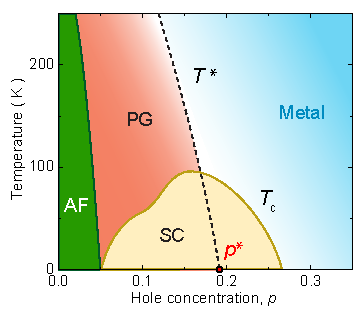
\includegraphics[width=0.5\textwidth]{figures/phase_diagram}
    \caption{Phase diagram of Cuprates. $p^*$ marks the QCP.}
    \label{fig:phase_diagram}
\end{figure}

The origin of high-temperature superconductivity in Cuprates is still the subject of intense
research and debate, but a possible explanation has to do with the Quantum Critical Point (QCP).
The QCP is a point in the phase diagram of a material where there is a phase transition at zero
temperature. This phase transition is driven by quantum effects, hence the name. In the case of
Cuprates, this is a critical doping level, usually denoted by $p_c$ or $p^*$. The actual existence
of a QCP for Cuprates is still a matter of debate and it is the subject of this project.

In their 2019 paper, Michon et al. \cite{michon2019} used secific heat measurements to
show the existence of the QCP. The effective mass of the charge carriers is expected to diverge at
the QCP, and the effective mass is proportional to $C/T$ where $C$ is the specific heat attributed
to the charge carriers and $T$ is the temperature. So, to probe the QCP, Michon et al. measured
the specific heat at very low temperatures (1 to 2 K) and extrapolated to zero temperature. More
specifically, they show
\begin{equation}
    \frac{C(T)}{T} = \gamma + \beta T^2.
\end{equation}
They found $\gamma$ peaks at the critical doping level, which is the signature of the QCP.